\chapter[Metodologia]{Metodologia}
A metodologia escolhida para o desenvolvimento do projeto será a metodologia ágil, mais especificamente será utilizado o Kanban. A escolha dessa metodologia se dá pelas seguintes características: o projeto será desenvolvido de maneira incremental, ou seja, ele poderá ser modificado no decorrer da implementação; a equipe consiste em apenas uma pessoa, o que descarta a possibilidade de utilizar o Scrum ou XP; o escopo do projeto será divididos em tarefas, e a utilização do Kanban facilita no descobrimento de gargalos.

A metodologia Kanban surgiu no Japão com o TPS\cite{tps} para controlar a fabricação de automóveis e foi inserida no meio de desenvolvimento de software no ano de 2007. Kanban é um termo japonês para sinal visual, uma das grandes características dessa metodologia é evidenciar os problemas existentes no processo. 

A metodologia ágil surgiu no ano de 2001, com a reunião de especialistas em processos de desenvolvimento de software para discutir maneiras de melhorar o desempenho em projetos, com isso foi criado o Manifesto Ágil\cite{agil}. Uma das características das metodologias ágeis são sua capacidade de adaptar a novos fatores durante o desenvolvimento do projeto, ao invés de tentar prever o que pode acontecer e o que não pode
\section{Requisitos}
Os requisitos do projeto serão classificados em três níveis de hierarquia:  épicos, features e user stories. Os épicos são compostos por features e representam macro entregáveis do projeto, geralmente são descritos como o nível mais abstrato. As features são agrupamentos de user stories e representam funcionalidades do sistema. User stories são pequenas partes de uma funcionalidade do sistema e que serão implementadas, user stories também podem ser classificadas como technical stories, estas technical stories representam atividades que não agregam muito valor ao cliente, porém elas agregam numa melhora interna no software.

No contexto do projeto as features serão equivalentes às milestones, e as stories (users ou technical) serão as issues. Para uma melhor visualização dos requisitos do projeto, será montado uma matriz de rastreabilidade para cada epico, sendo mostrado nas figuras \ref{image:ep01}, \ref{image:ep02} e \ref{image:ep03}.
\begin{figure}
\centering
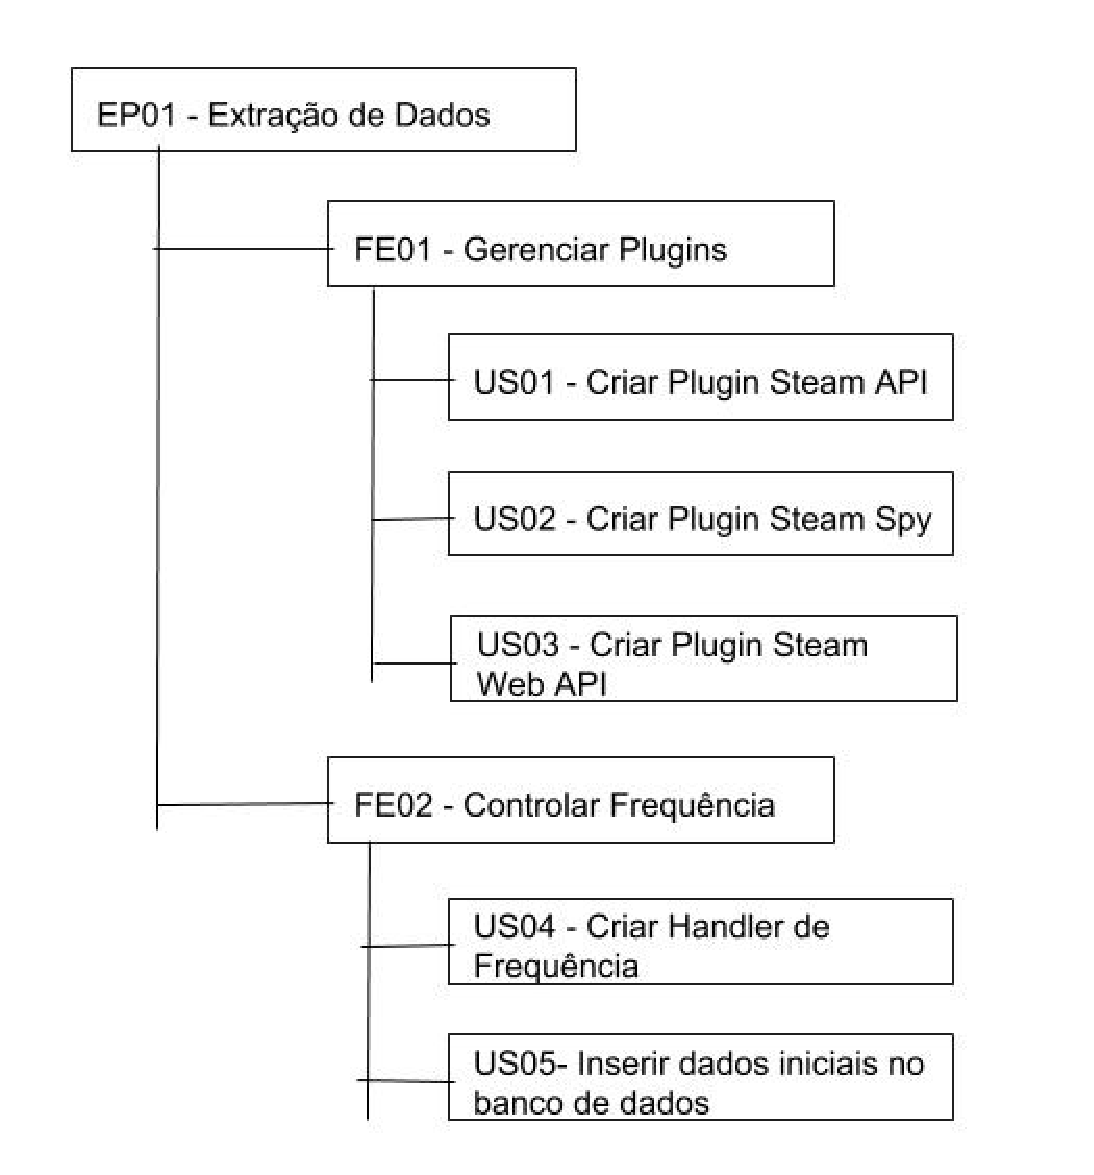
\includegraphics[scale=0.35]{figuras/EP01.eps}
\caption{Matriz Rastreabilidade Épico 1}
\label{image:ep01}
\end{figure}
\begin{figure}
\centering
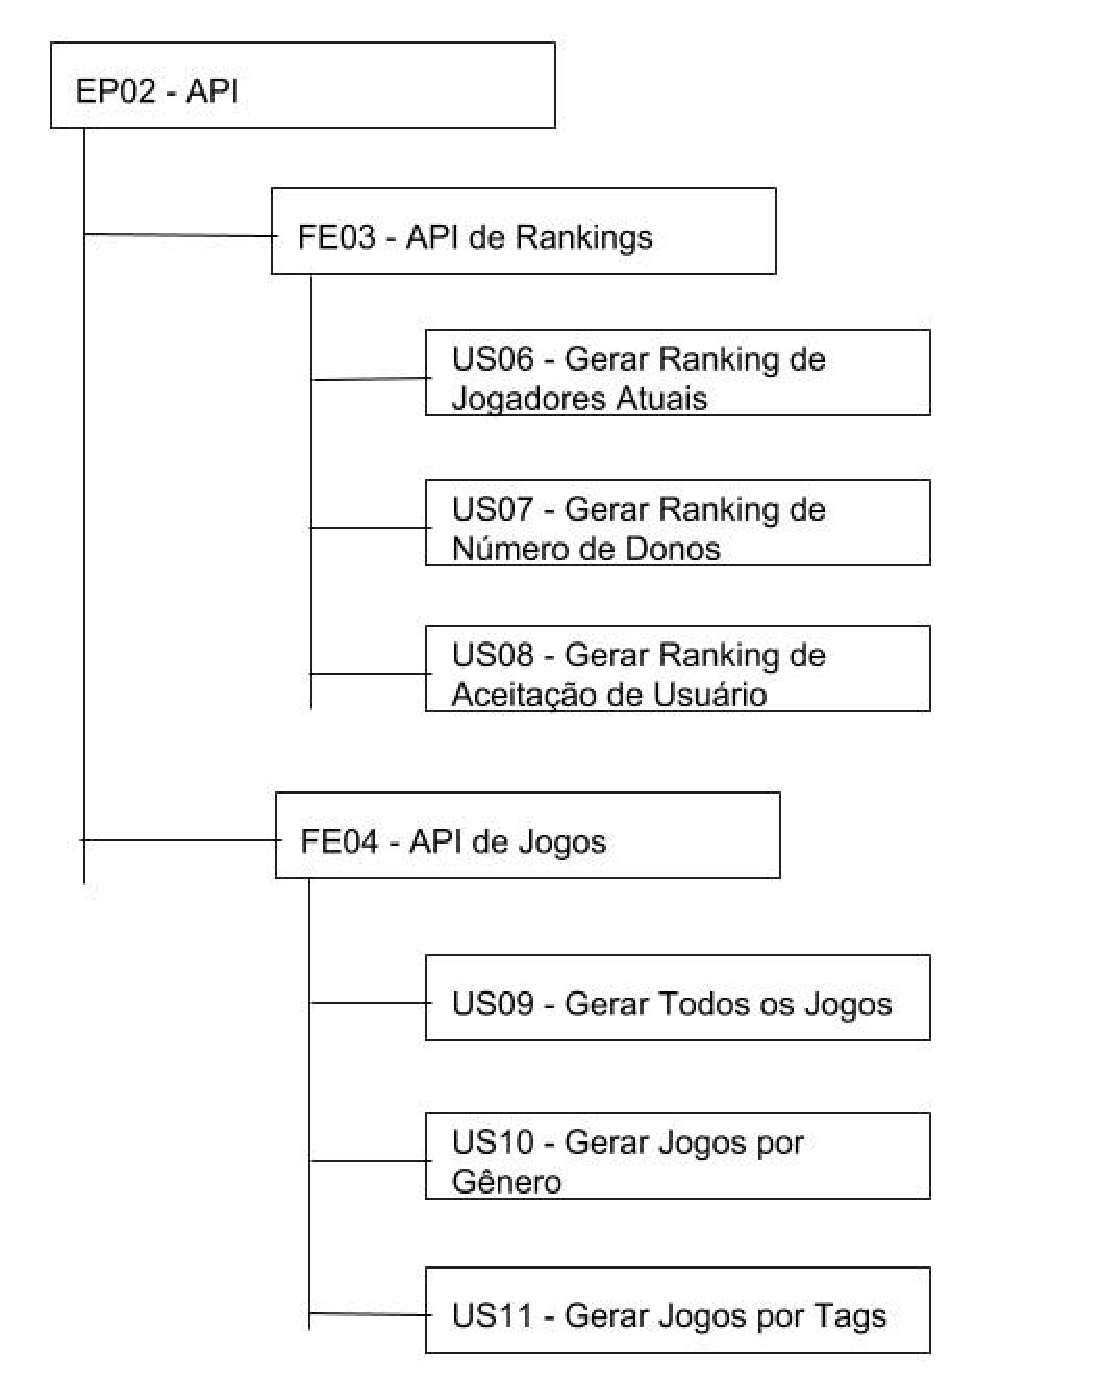
\includegraphics[scale=0.35]{figuras/EP02.eps}
\caption{Matriz Rastreabilidade Épico 2}
\label{image:ep02}
\end{figure}
\begin{figure}
\centering
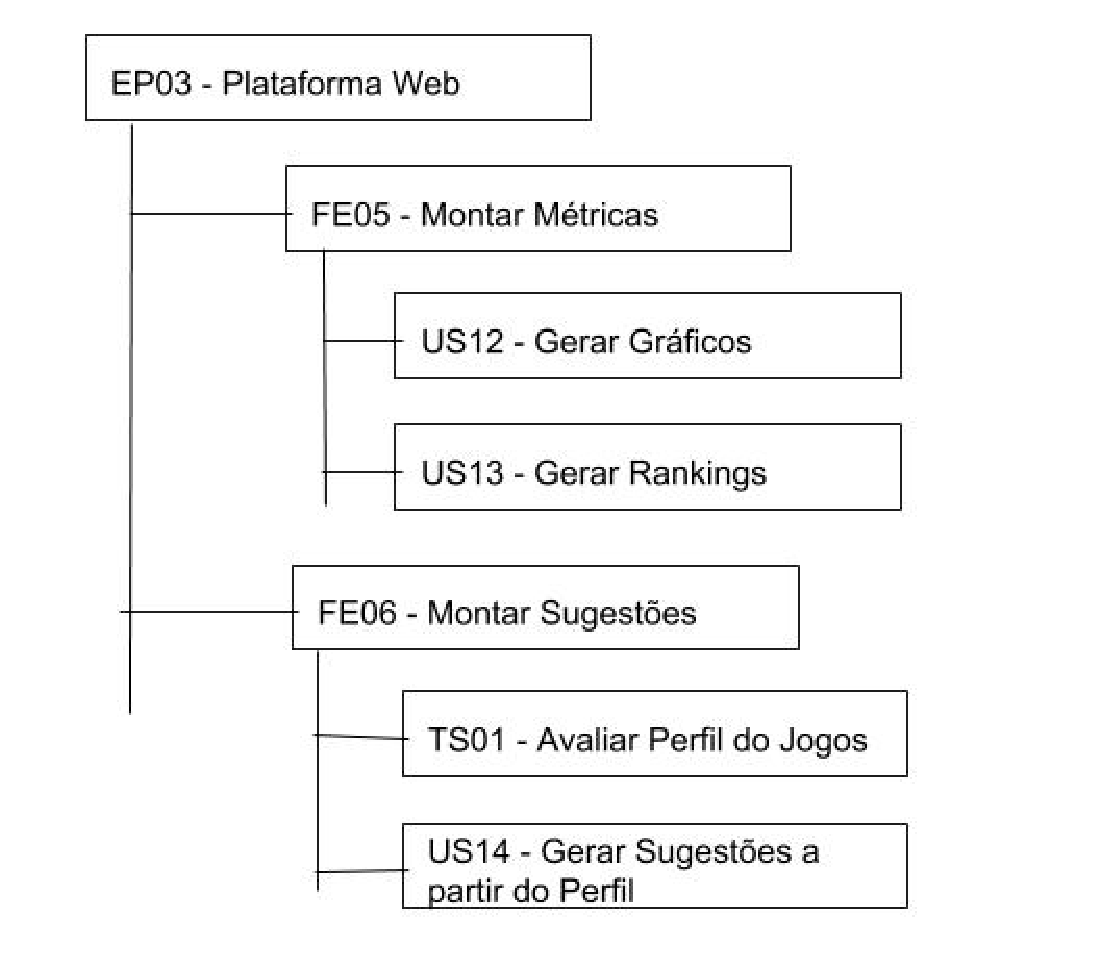
\includegraphics[scale=0.35]{figuras/EP03.eps}
\caption{Matriz Rastreabilidade Épico 3}
\label{image:ep03}
\end{figure}
\section{Arquitetura do Projeto}
A arquitetura do projeto é dividida principalmente em cinco partes, sendo elas: os logs, o software de extração, o banco de indexação, a API de consumo e a plataforma web. A ligação entre as partes e sua posição na arquitetura ficam evidenciado na figura \ref{image:arquitetura}.
\begin{figure}
\centering
\includegraphics[scale=0.3]{figuras/arquiteturaGeral.eps}
\caption{Arquitura Geral do Projeto}
\label{image:arquitetura}
\end{figure}
\subsection{Logs}
Logs é a parte onde se concentra os dados que serão utilizados para o desenvolvimento da plataforma web, como mostrado na figura, logs representam de onde virão os dados, sejam elas de um banco de dados, de uma função crawlers, de alguma API ou de um arquivo local.

Esses logs serão guardados e manipulados pelo software de extração. Para o escopo inicial do projeto serão utilizados três logs, sendo eles três APIs, a API do Steam Spy, a API do Steam Store e a API do Steam Web.
\subsection{Software de Extração}
O software de extração é dividido em três componentes principais, sendo eles: o handler, a classe main e os plugins. A arquitetura do software de extração e a interação entre seus componentes são demonstrados na figura \ref{image:extracao}.
\begin{figure}
\centering
\includegraphics[scale=0.35]{figuras/softwareExtracao.eps}
\caption{Arquitura do Software de Extração}
\label{image:extracao}
\end{figure}
A classe Main é responsável por criar o banco de indexação e fazer a primeira população necessária no mesmo. Como demonstrado na imagem da arquitetura do software de extração a classe main irá receber os dados para a primeira inserção dos plugins.

O handler é responsável por atualizar as informações no banco de indexação. Essas informações virão do plugin que além de mandar a informação deve indicar com que frequência esses dados devem ser atualizados.

Já os plugins são responsáveis por extrair os dados dos logs, manipulá-los caso seja necessário e enviar para o banco de dados. Para que o software de extração possua uma melhor organização, cada plugin só deve ser responsável por um tipo de log, pois assim permite que futuramente outros plugins sejam adicionados no software de extração.
\subsection{Banco de Indexação}
O banco de indexação será responsável por guardar os dados extraídos do log pelo software de extração. Como a Steam possui muito jogos, o banco de indexação que será usado deverá suportar um grande número de dados e também possuir uma rapidez na hora da busca. O banco de dados escolhido foi o Elasticsearch, por que além de suportar grandes quantidades de dados e ser rápido, ele também disponibiliza certa estatísticas sobre os dados e ser suportado por muitas linguagens de programação.
\subsection{API de Consumo}
A API de consumo é responsável principalmente por permitir que mais de uma plataforma possam utilizar seus dados. Está API irá consumir os dados do banco de indexação e a partir disso gerar links de API. Os principais links que serão desenvolvidos no escopo do projeto serão os de rankings e os de jogos.
\subsection{Plataforma Web}
A plataforma web é o principal componente da arquitetura, pois é nele que será mostrado as métricas levantadas para o auxilios das desenvolvedores. Está plataforma irá consumir os dados disponibilizados pela API, montar métricas em cima desses dados e disponibilizá-los de maneira que seja fácil a interpretação dos usuários. A plataforma também será responsável por montar pequenas sugestões para as desenvolvedoras.

\section{Software Extração}
O software de extração é a primeira parte propriamente dita que faz parte do projeto, nela é onde será feito a extração dos dados dos logs, a manipulação necessária e a inserção dos dados no banco de indexação numa determinada frequência. Primeiramente iremos falar sobre os logs. Logs, como já citados na arquitetura do projeto, são os arquivos que contém os dados que serão inseridos no banco de indexação. No escopo inicial serão utilizados três logs, sendo eles:
\begin{itemize}
	\item \textbf{Steam Web API}: É uma API REST disponibilizada pela Steamworks, ou seja, é uma API oficial da Steam\cite{steam_api}. Ela é uma API que possui tanto métodos públicos, tanto métodos privados. Os métodos públicos são abertos para qualquer pessoas visualizar, já os métodos privados é necessário uma chave de desenvolvedor cedido pela própria Steamworks. Para acessar seus dados é preciso, além da chave, a interface na qual aquele dados está guardado, o id do jogo, caso a informação seja de um jogo, ou do id do usuário, caso a informação seja de algum usuário.
	\item \textbf{Steam Store API}: É uma API REST disponibilizada pela Steam, que não possui uma página oficial para ela. Está API disponibiliza os dados dos jogos que estão guardados no banco de dados da Steam. Para acessar seus dados e preciso saber apenas o id do jogo, porém é possível passar filtros também.
	\item \textbf{Steam Spy API}: É uma API REST disponibilizada pelo Steam Spy\cite{steam_spy}, ela é muito parecido com a Steam Store API, porém ela disponibilizada dados que apenas o Steam Spy possui, como o número de donos de um jogo ou o número de avaliações positivas e negativas de um jogo. Para acessar seus dados é preciso saber apenas o id do jogo, porém também é possível passar filtros.
\end{itemize}
Com os logs definidos, é preciso saber quais dados dos logs serão inseridos no banco de indexação, pois muitas APIs possuem dados repetidos e nem todo os dados são interessante para se manter. Com isso os principais dados que serão mantidos no banco de indexação são:
\begin{itemize}
	\item \textbf{Nome}: É o nome do jogo em questão, este dado é guardado apenas para uma referenciação, pois ele não será utilizado na montagem das métricas.
	\item \textbf{Steam Id}: É o id do jogo, esse número é necessário pois é a partir dele que serão extraídas as informações das APIs.
	\item \textbf{Descrição}: É uma breve descrição sobre o jogo, este dado será guardado apenas para uma referenciação, pois ele não será utilizado na montagem das métricas.
	\item \textbf{Desenvolvedora}: É o nome da empresa que desenvolveu o jogo, este dado será guardado, pois será levantado o número de desenvolvedoras que são a própria publicadora.
	\item \textbf{Publicadora}: É o nome da empresa que publicou aquele jogo, este dado será guardado, pois será levantado o número de desenvolvedoras que são a própria publicadora.
	\item \textbf{Preço}: É o preço em reais daquele jogo, este dado será guardado, pois será levantando o preço médio que um jogo em determinado perfil geralmente têm.
	\item \textbf{Categorias}: São as categorias que aquele jogo abrange, geralmente são mostradas como características que aquele jogo têm, este dado será guardado, pois a partir de determinadas categorias que um determinado perfil de jogos, poderá levantar sugestões para a melhoria daquele perfil.
	\item \textbf{Gêneros}: São os gêneros daquele jogo, este dado será guardado, pois a partir de um determinado gêneros, novas métricas serão montadas.
	\item \textbf{Data de Lançamento}: É a data de lançamento daquele jogo, este dado será guardado, pois com ele será montado uma métrica de quais mês um jogo com um determinado perfil foi mais lançado.
	\item \textbf{Linguagens Suportadas}: São as línguas que aquele jogo suporta, este dado será guardados, pois será levantado quais linguagens um jogo com determinado perfil possui mais suporte.
	\item \textbf{Número de Donos}: É o número médio de donos que aquele jogo têm, este dado será guardado, pois será levantada uma média de númerod de donos que um determinado perfil atingiu.
	\item \textbf{Avaliações Positivas e Negativas}: São o número de avaliações positivas e negativas que um jogo têm, este dado será guardado pois com ele será possível determinar a porcentagem de avaliações positivas que um jogo teve, e com isso será levantado uma média desta porcentagem que um determinado perfil atingiu.
	\item \textbf{Número de Jogadores Atuais}: É o número de jogadores que estão jogando um determinado jogo naquele momento, este dado será guardado, pois com ele será possível gerar rankings de quais jogo de um determinado perfil estão sendo mais jogados.
\end{itemize}
Com os dados definidos, é preciso definir como será feito o software de extração. O software de extração será feito utilizando a linguagem de programação Ruby, com integração com o Elasticsearch. Para a atualização frequente dos dados será utilizado a gem Clockwork. A escolha do Ruby como linguagem de programação, se justifica pelo fato, que o integrante do projeto possui mais familiaridade com a linguagem.
\section{API de Consumo}
A API de consumo será responsável por consumir o banco de indexação, e partir dos dados gerar links RESTFUL para que qualquer aplicação possa utilizá-la. A API deverá atualizar seus links com a mesma frequência com o qual o software de extração atualiza o banco de indexação. Está API será desenvolvida utilizando o framework Ruby on Rails, isto se justifica pelo fato, que o integrante do projeto possui mais familiaridade com o framework.

A API será dividido em duas frentes principais, uma frente irá gerar links para pegar informações dos jogos, e a outro irá gerar links onde serão gerados rankings de jogos.

Os links de informações dos jogos poderá receber vários filtros, sendo os mais comuns: pegar todos os jogos disponíveis no banco de indexação, pegar todos os jogos de um ou mais gêneros, pegar todos os jogos com uma ou mais determinadas categorias.

Os links de rankings gerarão rankings a partir de determinados filtros, sendo os mais comuns: gerar um rankings pelos jogos mais jogados naquele momento, gerar um rankings com os jogos que possui as maiores porcentagens de avaliações positivas. A API também deverá gerar qualquer ranking com os filtros de gêneros e categorias, ou seja, deve-se gerar um ranking qualquer para um determinado perfil de jogo.
\section{Plataforma Web}
A Plataforma Web é a parte principal do projeto, nela é onde será mostrado as métricas que serão montadas a partir dos dados extraídos dos logs. A plataforma será desenvolvida em algum framework de JavaScript, retirando os dados da API de consumo.

Outra funcionalidade importante para a plataforma web é a habilidade de fazer sugestões a partir de um determinado perfil de jogo. As sugestões serão a priori simples, sendo as mais comuns, a adição de um gênero ou categoria no perfil, para que este tenha uma aumento no seus número de vendas ou no número da porcentagem de avaliações positivas.

As métricas que serão disponibilizadas inicialmente pela plataforma são:
\begin{itemize}
	\item Número total de jogos que atendam aquele determinado perfil. A figura \ref{image:num_total} é uma representação da métrica.
	\begin{figure}
	\centering
	
\includegraphics[scale=0.5]{figuras/num_jogos.eps}
	\caption{Número total de jogos}
	\label{image:num_total}
	\end{figure}
	\item Número médio de donos que um jogo que atende aquele determinado perfil. A figura \ref{image:med_donos} é uma representação da métrica.
	\begin{figure}
	\centering
	
\includegraphics[scale=0.5]{figuras/media_donos.eps}
	\caption{Número médio de donos}
	\label{image:med_donos}
	\end{figure}
	\item Média das porcentagens de avaliações positivas de um jogo que atende aquele determinado perfil. A figura \ref{image:avaliacoes} é uma representação da métrica.
	\begin{figure}
	\centering
	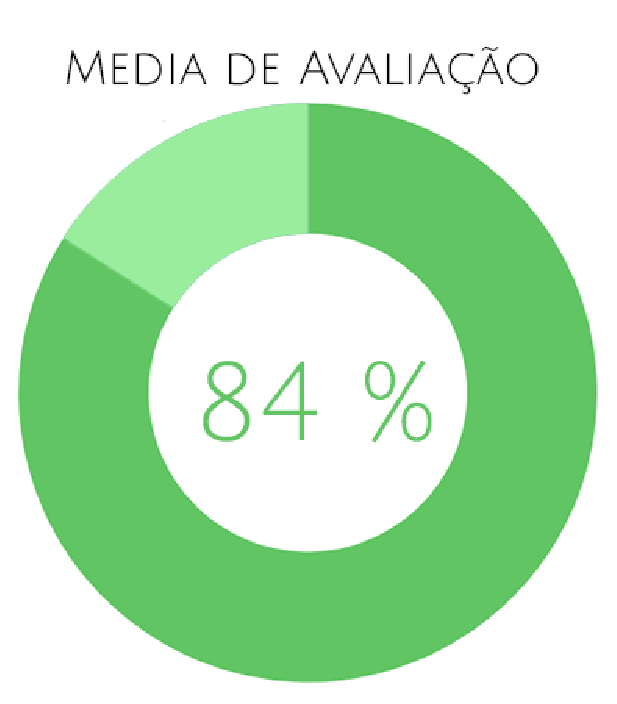
\includegraphics[scale=0.3]{figuras/avaliacao.eps}
	\caption{Média das porcentagens de avaliações positivas}
	\label{image:avaliacoes}
	\end{figure}
	\item Mês que possui o maior número de lançamento que atendam aquele determinado perfil. A figura \ref{image:mes} é uma representação da métrica.
	\begin{figure}
	\centering
	
\includegraphics[scale=0.5]{figuras/mes.eps}
	\caption{Mês com mais lançamentos}
	\label{image:mes}
	\end{figure}
	\item Gráfico de lançamentos por mês que atendam aquele determinado perfil. A figura \ref{image:lancxmes} é uma representação da métrica.
	\begin{figure}
	\centering
	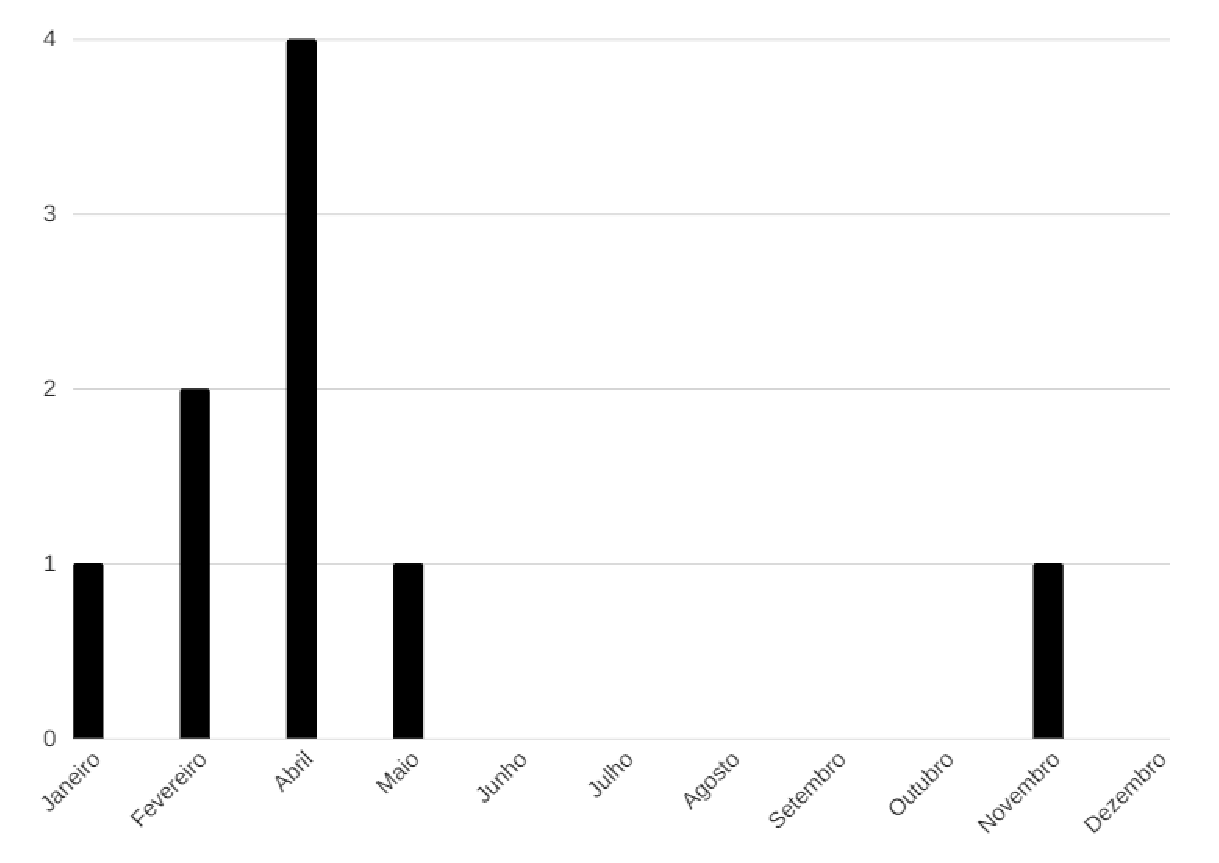
\includegraphics[scale=0.4]{figuras/lancamentoxmes.eps}
	\caption{Lançamentos x Mês}
	\label{image:lancxmes}
	\end{figure}
	\item Preço médio de um jogo que atende aquele determinado perfil. A figura \ref{image:preco} é uma representação da métrica.
	\begin{figure}
	\centering
	
\includegraphics[scale=0.5]{figuras/preco_medio.eps}
	\caption{Média dos preços}
	\label{image:preco}
	\end{figure}
	\item Número de jogos que foram publicados pela própria desenvolvedora que atendam aquele determinado perfil. A figura \ref{image:own} é uma representação da métrica.
	\begin{figure}
	\centering
	
\includegraphics[scale=0.5]{figuras/own_publisher.eps}
	\caption{Número de jogos publicados pela propria desenvolvedora}
	\label{image:own}
	\end{figure}
	\item Número de jogos que foram publicado por outra empresa que atendam aquele determinado perfil. A figura \ref{image:another} é uma representação da métrica.
	\begin{figure}
	\centering
	
\includegraphics[scale=0.5]{figuras/another_publisher.eps}
	\caption{Número de jogos publicados por outra empresa}
	\label{image:another}
	\end{figure}
	\item Gráfico que compara os números de jogos que foram publicados pela desenvolvedora pelo números de jogos que foram publicados por outra empresa por ano. A figura \ref{image:anotherxown} é uma representação da métrica.
	\begin{figure}
	\centering
	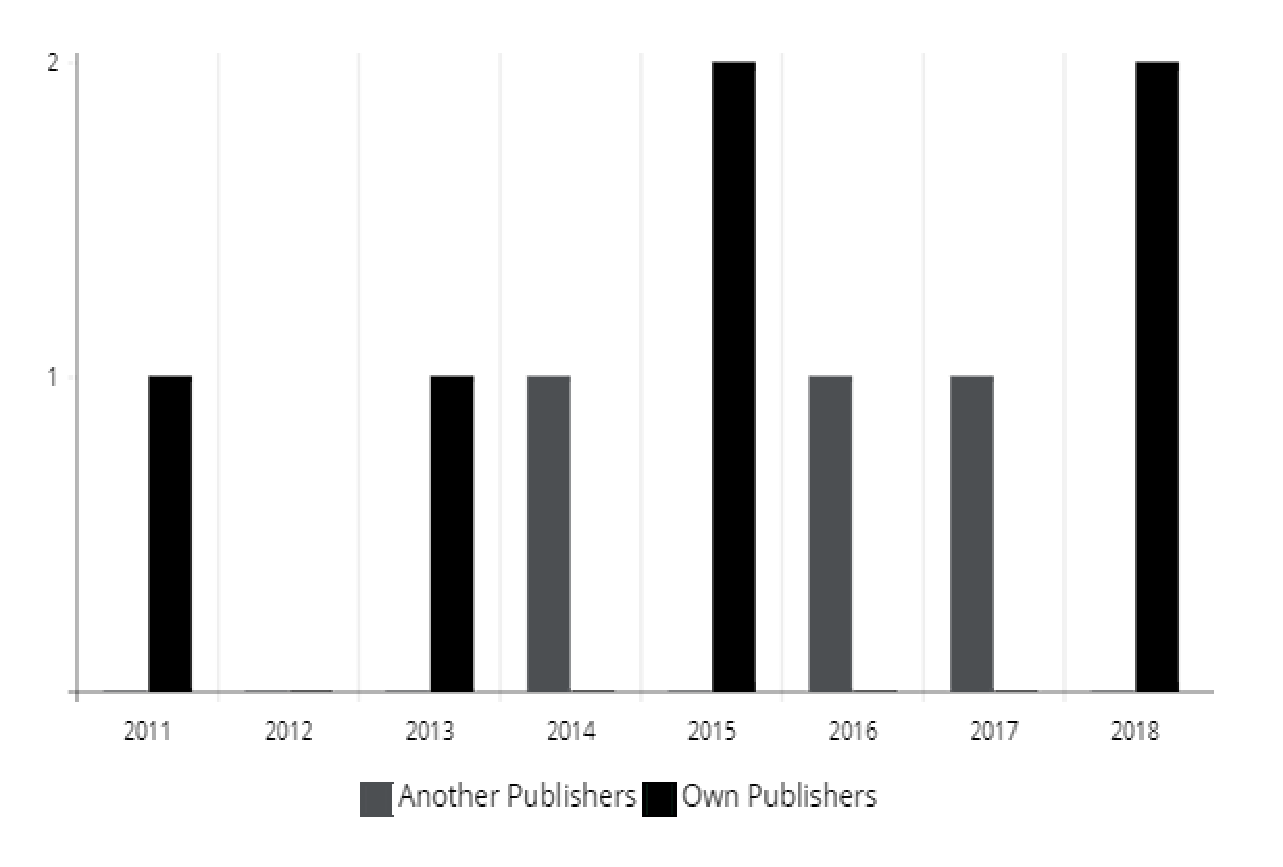
\includegraphics[scale=0.4]{figuras/anotherxown.eps}
	\caption{Outra Publicadora x Própria Desenvolvedora}
	\label{image:anotherxown}
	\end{figure}
	\item Tabela de quantos jogos daquele determinado perfil atingiram um número N de donos e sua porcentagem. A representação desta tabela fica evidenciada pela tabela \ref{table:num_donos}.
	\item Tabela de quantos jogos daquele determinado perfil atingiram um número N de avaliações positivas e sua porcentagem. A representação desta tabela fica evidenciada pela tabela \ref{table:avaliacao}
	\item Gráfico de desenvolvedoras por número de jogos desenvolvidos. A figura \ref{image:developers} é uma representação da métrica.
	\begin{figure}
	\centering
	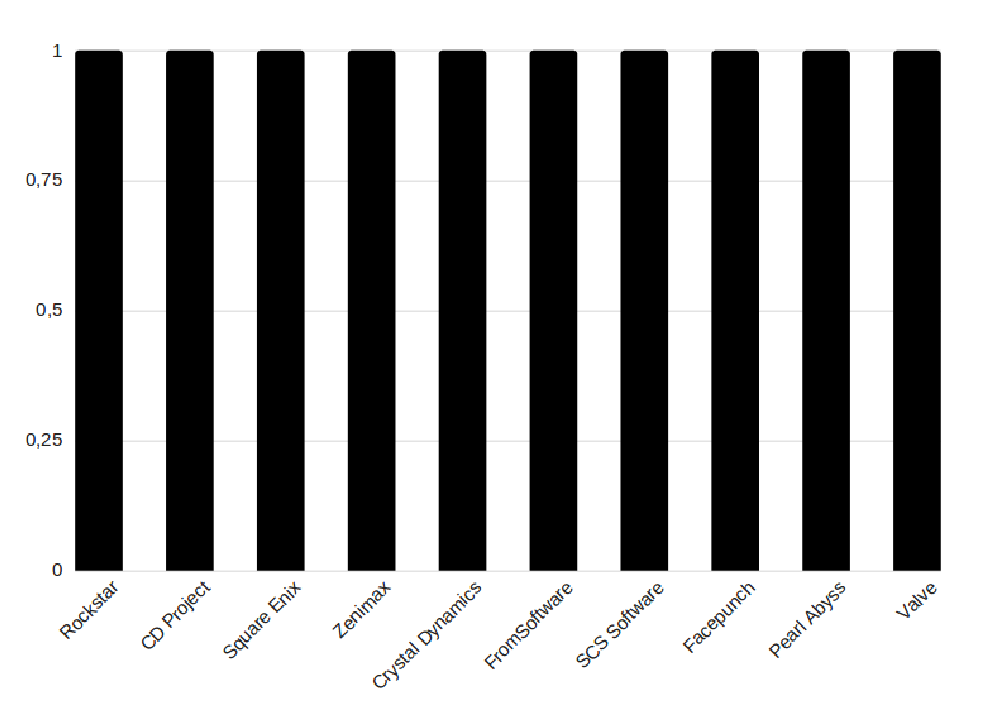
\includegraphics[scale=0.4]{figuras/developer.eps}
	\caption{Desenvolvedoras x Número de Jogos}
	\label{image:developers}
	\end{figure}
	\item Gráfico de linguangens suportados por número de jogos que a suportam. A figura \ref{image:languages} é uma representação da métrica.
	\begin{figure}
	\centering
	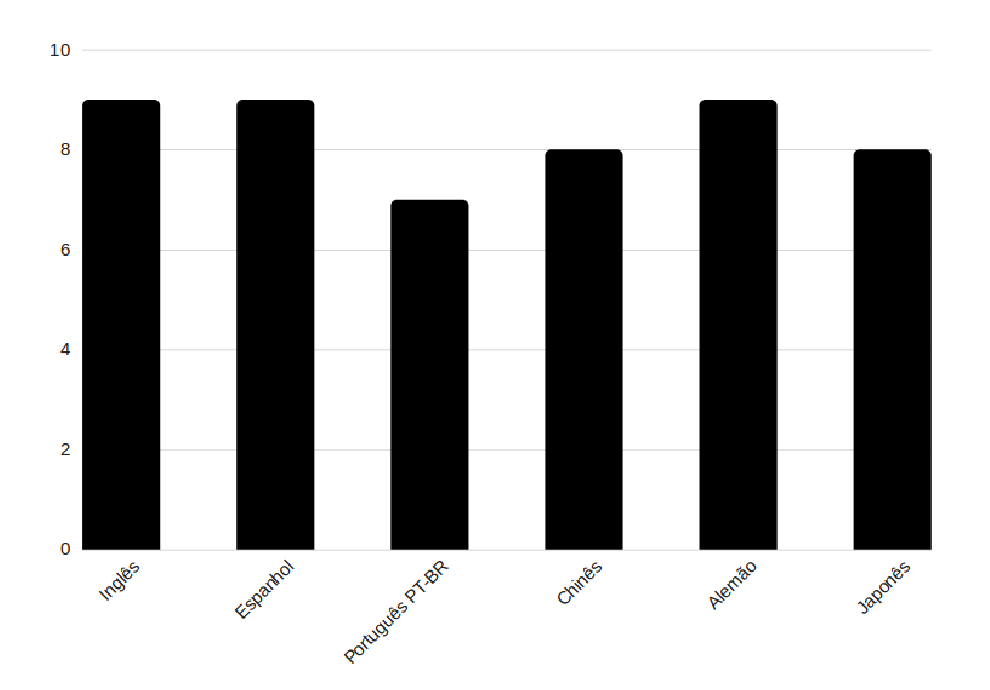
\includegraphics[scale=0.4]{figuras/language.eps}
	\caption{Linguagens Suportados x Número de Jogos}
	\label{image:languages}
	\end{figure}
\end{itemize}
\begin{table}
\centering
\begin{tabular}{|p{5cm}|p{5cm}|p{5cm}|}
\hline \textbf{Número de Donos} & \textbf{Quantidade de Jogos} & \textbf{\% de Jogos} \\
\hline 0 - 10000 & 10 & 100 \% \\
\hline 10000 - 50000 & 10 & 100 \% \\
\hline 50000 - 100000 & 9 & 90 \% \\
\hline 100000 - 500000 & 9 & 90 \% \\
\hline 500000 - 1000000 & 9 & 90 \% \\
\hline 1000000 - 5000000 & 8 & 80 \% \\
\hline 5000000 - 10000000 & 3 & 30 \% \\
\hline 10000000 - 50000000 & 1 & 10 \% \\
\hline
\end{tabular}
\caption{Número de donos e sua porcentagem}
\label{table:num_donos}
\end{table}
\begin{table}
\centering
\begin{tabular}{|p{5cm}|p{5cm}|p{5cm}|}
\hline \textbf{Porcentagem de Avaliação} & \textbf{Quantidade de Jogos} & \textbf{\% de Jogos} \\
\hline 0 \%- 10 \% & 10 & 100 \% \\
\hline 11 \%- 20 \% & 10 & 100 \% \\
\hline 21 \%- 30 \% & 10 & 100 \% \\
\hline 31 \%- 40 \% & 10 & 100 \% \\
\hline 41 \%- 50 \% & 10 & 100 \% \\
\hline 51 \%- 60 \% & 10 & 100 \% \\
\hline 61 \%- 70 \% & 10 & 100 \% \\
\hline 71 \%- 80 \% & 8 & 80 \% \\
\hline 81 \%- 90 \% & 6 & 60 \% \\
\hline 91 \%- 100 \% & 4 & 40 \% \\
\hline
\end{tabular}
\caption{Porcentagem de avaliação}
\label{table:avaliacao}
\end{table}